\chapter{Aspecte teoretice}

\section{Preambul}

În domeniul probabilităților un model Markov este folosit pentru a modela un sistem ce se schimbă într-un mod aleator. De obicei acesta ține cont doar de starea curentă și nu depinde de evenimentele anterioare, acest lucru numindu-se și prorietatea Markov. Ulterior s-au dezvoltat modele ce au un așa numit ordin, extinzând astfel numărul de stări de care se ține cont în cadrul modelului.\par

De obicei există o separare clară între tipurile de modele Markov, criteriul folosit este disponibilitatea de a observa sau nu stările modelului. Așadar rezultă două mari categorii, sisteme cu stări complet observabile, din care fac parte lanțurile Markov și sisteme cu stări parțial observabile, cel mai cunoscut sistem fiind modelul Markov cu stări invizibile sau \textbf{HMM} \footnote{Hidden Markov Model}. Pe langă aceste sistem prezentate, s-au dezvoltat și anumite derivate fiecare cu avantajele sale demonstrând astfel flexibilitatea și capacitatea de modelare a acestor sisteme.\par

În mare parte această teză se axează în jurul parții discrete a acestor modele, numărul de stări/observații find finit numărabile și ușor de caracterizat dar există și o ramură ce se ocupă cu partea continuă, fiecare abordare avănd avantajele și dezavantajele ei.\par

Legat de partea practică, de-a lungul timpului aceste sisteme au fost folosite în foarte multe domenii de la bioinformatică până la lingvistică computațională. O aplicație foarte importantă a acestor modele este recunoașterea vocală, modelele Markov fiind standardul folosit în industrie pentru asistenții personali ca \textit{Siri} și \textit{Alexa}.\par

\section{Modele Markov cu stări invizibile}

Acest model statistic este caracterizat în principal de faptul că stările interne sunt ascunse de un privitor exterior. Tot ce se poate observa în cadrul acestui model este emisia unor etichete sau obiecte 
$\{V_{1},V_{2},V_{3},\dots,V_{n}\}$ dintr-o mulțime notată pe scurt $V$. Acest lucru complică în general structura modelului și algortimii ce folosesc acest sistem. \par

Un avantaj direct este creșterea capacității de expresivitate, putând modela mai fidel datele, datorită eliminării necesității de a cunoaște toate stările evenimentului.\par

Pentru a caracteriza concret și complet acest model avem nevoie de un \textit{5-uplu} $ HMM = (\textbf{S},\textbf{V},\textbf{A},\textbf{B},\pi)$ ce desemnează astfel : \par
\begin{itemize}
\item{$\textbf{S} = \{S_{1},S_{2},\dots,S_{N}\}$ mulțimea ce desemnează numărul de stări ascunse din model, avand un numar de $N$ elemente. Starea relativă la timpul $t$ se va nota ca și $q_{t}$.}
\item{$\textbf{V} = \{V_{1},V_{2},\dots,V_{M}\}$ , cele $M$ etichete observabile.}
\item{$\textbf{A} = \{a_{ij}\}$ unde $a_{i,j} = P(q_{t+1} = S_{j} | q_{t} = S_{i}) , 1 \leq i , j \leq N$ , reprezentând distribuția de probabilitea asociată tranzițiilor între stări.}
\item{$\textbf{B} = \{b_{i}(k)\}$ unde $b_{i}(k) = P(V_{k}\ la\ timpul\ t\ | q_{t} = S_{i}), 1 \leq i \leq N , 1 \leq k \leq M$, reprezentând distribuția de probabilitate asociată emiterii unui element din $V$ în starea $i$.}
\item{$\pi = \{\pi_{i}\}$ unde $\pi_{i} = P(q_{1} = S_{i}) , 1 \leq i \leq N$, folosit inițial pentru a stabili prima stare din model și anume $q_{1}$.}
\end{itemize}
\par

În general modul de funcționare a acestui model poate fi descris foarte ușor cu o porțiune de pseudocod:

\begin{lstlisting}[mathescape=true , caption=Pseudocod ce descrie modul de operare a unui $HMM$]
t $\gets$ 1;
stare $\gets$ alege o stare $S_{i}$ cu probabilitate $\pi_{i}$;
repeta la infinit
	stare $\gets$ alege o noua stare $S_{j}$ de tranzitie de la starea $S_{i}$ cu probabilitate $a_{ij} \in \textbf{A}$;
	afiseaza observatia $V_{k}$ cu probabilitatea $b_{i}(k)\in \textbf{B}$;
	t $\gets$ t + 1;
\end{lstlisting}

Uneori printre alte publicații de specialitate modelul poate fi descris prin specificarea parametrilor $N,M$ și cele trei distribuții de probabilitate notate astfel $\lambda = \{\textbf{A},\textbf{B},\pi\}$.\par
\vspace{10mm}
\begin{figure}[H]
\centering
\begin{tikzpicture}
  \node[box,draw=white!100] (Latent) {\textbf{Stări latente}};
  \node[main] (L1) [right=of Latent] {$q_{1}$};
  \node[main] (L2) [right=of L1] {$q_{2}$};
  \node[main] (L3) [right=of L2] {$q_{3}$};
  \node[main] (Lt) [right=of L3] {$q_{t}$};
  \node[main,fill=black!10] (O1) [below=of L1] {$v_{1}$};
  \node[main,fill=black!10] (O2) [below=of L2] {$v_{2}$};
  \node[main,fill=black!10] (O3) [below=of L3] {$v_{3}$};
  \node[main,fill=black!10] (Ot) [below=of Lt] {$v_{t}$};
  \node[box,draw=white!100,left=of O1] (Observed) {\textbf{Etichetele emise}};
  \path (L3) -- node[auto=false]{\ldots} (Lt);
  \path (L1) edge [connect] (L2)
        (L2) edge [connect] (L3)
        (L3) -- node[auto=false]{\ldots} (Lt);
  \path (L1) edge [connect] (O1);
  \path (L2) edge [connect] (O2);
  \path (L3) edge [connect] (O3);
  \path (Lt) edge [connect] (Ot);
\end{tikzpicture}
\caption{Modul de funcționare a modelului Markov cu stări invizibile}
\end{figure}
\par

În cadrul aplicației mulțimea de etichete \textbf{V} au fost reprezentată de elementele de tip \textit{GameObject} ce urmează a fi instanțiate. Din motive de performanță și flexibilitate, aplicația folosește în total un număr de sașe modele Markov cu stări invizibile a căror parametri au fost estimați să respecte anumite restricții.\par

Se poate face o distincție între cei șase generatori după scopul lor în cadrul jocului, trei dintre ei sunt folosiți pentru a genera terenul pe care jucătorul navighează. Această decizie a fost facută din necesitatea de a putea controla numărul de platforme pentru fiecare din cei trei generatori, ce în fond reprezintă trei zone distincte, urbană, rurală și deșertică enumerate conform ordinii de apariție în joc.\par

\vspace{10mm}
\begin{figure}[H]
\centering
\begin{tikzpicture}

  \node[main] (L1) {$S_{1}$};
  \node[main] (L2) [right=of L1] {$S_{2}$};
  \node[main] (L3) [right=of L2] {$S_{3}$};
  \node[main] (L4) [right=of L3] {$S_{4}$};
 \node[main] (L5) [right=of L4] {$S_{5}$};
  \node[main] (S) [above=2cm of L3]{$S$};

  \node[main,fill=black!10] (V) [below=2cm of L3] {$V$};
  \path (L1) edge [connect,bend right=45] (L2);
  \path (L2) edge [connect, bend right=45] (L3);
  \path (L3) edge [connect, bend right=45] (L4);
  \path (L4) edge [connect, bend right=45] (L5);
  \path (L2) edge [connect,bend right=45] (L1);
  \path (L3) edge [connect, bend right=45] (L2);
  \path (L4) edge [connect, bend right=45] (L3);
  \path (L5) edge [connect, bend right=45] (L4);
  \path (L1) edge [connect, bend right=30] (V);
  \path (L2) edge [connect, bend right=30] (V);
  \path (L3) edge [connect,] (V);
  \path (L4) edge [connect, bend left=30] (V);
 \path (L5) edge [connect, bend left=30] (V);
 \path(S) edge[connect, bend right=30] (L1);
 \path(S) edge[connect, bend right=30] (L2);
 \path(S) edge[connect] (L3);
 \path(S) edge[connect, bend left=30] (L4);
 \path(S) edge[connect, bend left=30] (L5);
\end{tikzpicture}
\caption{Structura orientativă a unui generator}
\end{figure}
\par

Se observă din figură, că avem un nod de start \textbf{S} ce ne conduce la una dintre cele cinci stări, iar fiecare stare are acces la \textbf{V}, mulțimea etichetelor, în cazul nostru la cele trei tipuri de platformă \textit{Left},\textit{Right} și \textit{Straight}. Din model s-au omis probabilitățile de pe arce tocmai pentru a nu încărca desenul căt și pentru faptul că ele vor fi stabilite ulterior de un algoritm de estimare a parametrilor, inițial probabilitățile fiind generate aleator.\par

Restul generatorilor sunt folosiți pentru obiectele ce urmează a popula platformele. Din cauza complexității și a numărului mare de stări și etichete nu se poate realiza o reprezentare grafică. Cel mai mare dintre generatori are douăzeci de stări și zece obiecte ce au rol de etichete pentru emisie.\par

O observație importantă legată de mulțimea \textbf{V} este că aceasta conține un element mai special și anume un \textit{GameObject} denumit sugestiv epsilon. Acest obiect semnifică elementul vid, prin care se poate insera un spațiu între obiectele din scenă pentru un aspect mai plăcut la instanțierea pe platforme. Această decizie s-a luat din necesitatea de a separa unele obiecte de celelalte pentru a putea reproduce mai fidel lumea reală.\par

\section{Estimare de parametri}

Această dilema este una dintre cele trei mari aspecte a modelelor Markov cu stări invizibile, celelalte două fiind determinarea probabilității de emisie a unei secvențe și determinarea celei mai bune secvențe de stări ce descriu seria de emisii observate. Problema estimării de parametri este cea mai grea dintre cele trei, nici până în momentul de fața nu s-a dezvoltat un algoritm simplu ce rezolvă această problemă. Majoritatea algoritmilor folosesc o metodă iterativă pentru a incerca o estimare a parametrilor ce descriu un \textbf{HMM} și anume $\lambda = \{\textbf{A},\textbf{B},\pi\}$.\par

Din cauză naturii iterative în general acești algoritmi se bazează pe aproprierea față de un anumit punct pentru terminare. Un lucru bun este că s-a demonstrat proprietatea de convergență a acestor algoritmi, ceea ce inseamnă că se termină întotdeauna, cu toate acestea abordarea iterativă suferă de o convergență foarte înceată și de pericolul continuu de a rămâne blocat într-un optim local.\par

De aceea s-au încercat multe artificii pentru a obține un $log-likelihood$ căt mai bun. Unul dintre ele, folosit și de această aplicație, este inițializarea aleatoare a parametrilor $\lambda = \{\textbf{A},\textbf{B},\pi\}$ și incercarea antrenării până la convergență de mai multe ori pastrăndu-se cel mai bun rezultat. De asemenea numărul de stări latente poate influența drastic comportamentul modelului, fiind un factor decisiv între $underfit$ și $overfit$.\par

Din păcate determinarea acestui număr de stări optim pentrun un model dat este o problemă grea ce nu are o soluție fixă. În general abordarea acestei probleme este prin $trial\ and\ error$. Există și anumite criterii bazate pe $log-likelihood$ și numărul parametrilor din model, cum ar fi $BIC$ \footnote{Bayesian Information Criterion} sau $AIC$ \footnote{Akaike Information Criterion}.\par

În cadrul acestei proiect a fost folosită metoda $trial\ and\ error$ în defavoarea criteriilor prezentate mai sus doarece, modelele sunt relativ mici și nu necesită cei mai optimi parametri. În general s-a urmărit ca numărul de stări să fie mai mare decăt numărul de etichete, ceea ce previne de fapt inabilitatea rețelei de a învăța restricțiile la antrenare. Acest lucru se mai numește și $underfit$.\par

\section{Algoritmi pentru estimare de parametri}

Cel mai cunoscut algoritm pentru inferare de parametri, fiind dat un model Markov cu stări invizibile este așa numitul algoritm \textbf{Baum-Welch} sau algoritmul \textbf{Forward-Backward}. Așa cum implică și numele acest algoritm are la bază două etape. Inițial parametri modelului $\lambda = \{\textbf{A},\textbf{B},\pi\}$ sunt inițializați aleator și mai apoi actualizați după fiecare iterație până la convergență după cum urmează:
\begin{itemize}
\item{\textbf{Forward} este etapa în care se calculează de obicei $P(O|\lambda)$, unde $O$ este secvența de etichete observate, folosind tehnica programării dinamice pentru stocarea anterioară a rezultatelor. Acest calcul este necesar doarece va fi folosit în urmatoarea etapă pentru reajustarea parametrilor modelului.}
\item{\textbf{Backward} este etapa de calcul a probabilității $P(O_{t+1},\dots,O_{T}| S_{i},\lambda)$, unde $T$ este lungimea de etichete observate, ceea ce semnifică șansa de a observa secvența $O_{t+1},\dots,O_{T}$ aflându-ne în starea $i$ și la momentul $t$ din timp}.
\end{itemize}
\par

În ciuda popularității acestui algoritm am decis să folosesc altă modalitate de estimare a parametrilor din motive de viteză și simplitate atăt la nivel de implementare căt și la nivel teoretic. Acest algoritm ce estimează parametri modelului$^{\mathbf{[1]}}$ prezintă avantaje substanțiale asupra vitezei atunci cănd lungimea secvenței observate $O$ depășeste numărul de etichete posibile al modelului.\par

Un alt aspect alt acestei abordări este că algoritmul actualiează doar parametri $\textbf{A},\textbf{B}$ ai modelului ignorând complet parametrul $\pi$ ceea ce duce la o amplificare a vitezei cu consecințe minime, parametrul $\pi$ find folosit doar la alegerea stării inițiale $q_{1}$.\par

De asemenea ca și \textbf{Baum-Welch}, fiind dată o secvență $O$ de etichete observate de lungime $T$, antrenare nu se poate face pe o subsecvență $O_{1},\dots,O_{m}$ iar mai apoi pe o alta subsecvență $O_{m+1},\dots,O_{T}$, cu $1 \leq m \leq T$, deoarece modelul ar avea parametri adaptați doar după ultima subsecvență pe care a fost antrenat. Un alt aspect important este normalizarea valorilor ce se face la fiecare iterație după actualizarea parametrilor. Acest lucru este necesar doarece fiecare tranziție și emisie depinde în fond de o variabilă aleatoare a carei sumă de probabilități trebuie să fie exact egală cu unu.\par

Algoritmul pe care am decis să îl folosesc, deși foarte similar cu \textbf{Baum-Welch}, are la bază o matrice $C$ de dimensiune $M\times M$ construită cu scopul de a caracteriza numărul de apariții a unei anumite perechi $O_{t}O_{t+1}$ în secvența de etichete observate $O$.\par

Mai jos sunt prezentate câteva histograme ce modelează etichetele observate împreună cu perechile de etichete folosite la construirea matricei de frecvență.\par

\vspace{10mm}
\begin{figure}[H]
\centering
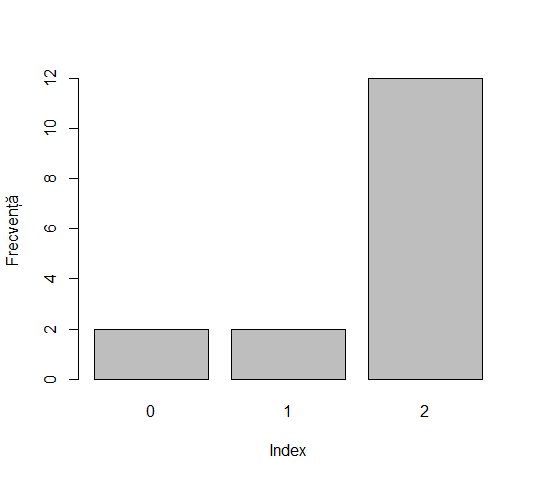
\includegraphics[width=0.75\linewidth]{CityPlatformPlot.png} \par
\caption{Histogramă a etichetelor pentru generatorul de platforme}
\end{figure}

\vspace{10mm}
\begin{figure}[H]
\centering
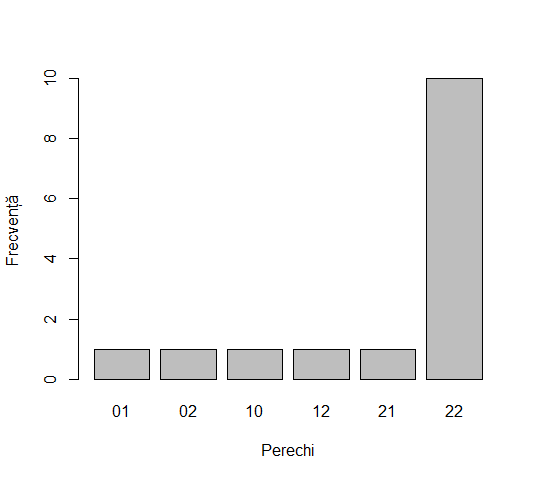
\includegraphics[width=0.75\linewidth]{CityPlatformPairPlot.png} \par
\caption{Histogramă a perechilor de etichete pentru generatorul de platforme}
\end{figure}

\vspace{10mm}
\begin{figure}[H]
\centering
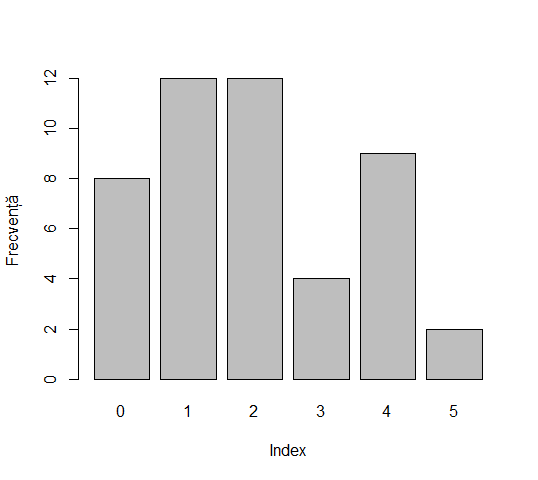
\includegraphics[width=0.75\linewidth]{DesertPropsPlot.png} \par
\caption{Histogramă a etichetelor folosite pentru generatorul de obiecte}
\end{figure}


\vspace{10mm}
\begin{figure}[H]
\centering
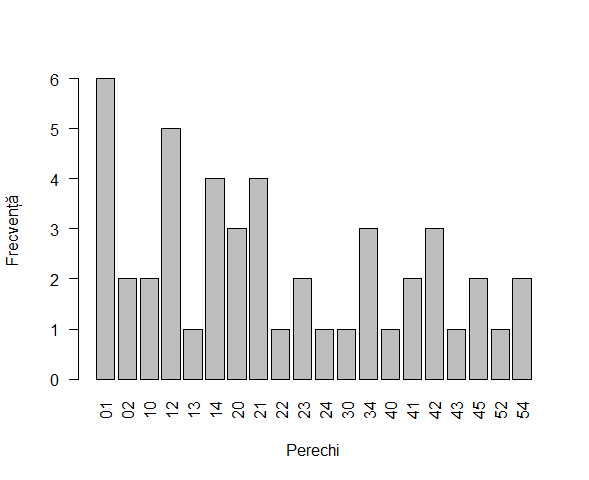
\includegraphics[width=0.75\linewidth]{DesertPropsPairPlot.png} \par
\caption{Histogramă a perechilor de etichete pentru generatorul de obiecte}
\end{figure}

Această soluție se bazează foarte mult pe calculul matriceal de accea în cadrul aplicației am fost nevoit să apelez la o librărie ce este folosită pentru calcul numeric. Deoarece acest algoritm se bazează foarte mult pe matrici, o incercare de implementare folosind unități de procesare grafice ar putea îmbunătăți substanțial viteza de convergență a algoritmului datorită puterii mai mari de calcul.\par

\begin{lstlisting}[mathescape=true, caption=Pseudocod ce descrie algoritmul de inferență]
Intrare: Matricea $\mathbf{C}, \mathbf{\bar{A}} , \mathbf{B^T}$
repeta pana la convergenta:
	$\mathbf{R} \gets \mathbf{C}  \oslash \mathbf{\bar{C}}$
	$\mathbf{\bar{A'}} \gets \mathbf{\bar{A'}} \odot (\mathbf{B^TRB})$
	$\mathbf{B'} \gets \mathbf{B} \odot (\mathbf{RB\bar{A^T}} + \mathbf{R^TB\bar{A}})$
	$\mathbf{\bar{A}} \gets norm(\mathbf{\bar{A'}})$
	$\mathbf{B} \gets norm(\mathbf{B'})$
$\mathbf{A} \gets norm(\mathbf{\bar{A'}})$
\end{lstlisting}

Parametri $\textbf{A},\textbf{B},\pi$ sunt initializați aleator și normalizați pe linii, iar apoi este calculat $\mathbf{\bar{C} = B\bar{A}B^{T}}$, unde $\mathbf{\bar{A}} = {\pi_{k}\cdot a_{kl}}, 1 \leq k \leq N, 1\leq l \leq N$. Următorul pas este calcularea matricii \textbf{R} prin împărțirea element cu element a matricii \textbf{C} la matricea $\mathbf{\bar{C}}$, notat cu $\oslash$ în cadrul pseudocodului.\par

După calculul acestor matrici intermediare urmează actualizare paremetrilor după urmatoarele ecuații$^{\mathbf{[1]}}$, $\mathbf{\bar{A'} = \bar{A} \odot B^{T}RB}$ și $\mathbf{B'} = \mathbf{B} \odot \mathbf{(RB\bar{A}^{T} + R^{T}B\bar{A})}$, unde $\odot$ reprezintă înmulțirea element cu element a două matrici. După acest calcul se face actualizarea astfel $\mathbf{A} = norm(\mathbf{\bar{A'}}),\mathbf{B} = norm(\mathbf{B'})$, unde $norm$ este o funcție ce realizează normalizarea pe toată matricea \textbf{A} iar pentru \textbf{B} doar pe coloane. De asemena se realizează și o normalizare a matricii \textbf{A} pe linii, la finalul iterațiilor.\par

Acești pași se realizează până un anumit set de criterii de convergență sunt satisfăcute. De obicei aceste criterii includ ca norma matricilor \textbf{A,B} să fie sub un anumit epsilon împreună cu funcția de $log-likelihood$. În implementarea acestui algoritm am folosit ca și criterii de convergență, sugerate pentru algoritmul descris mai sus$^{\mathbf{[1]}}$, calcularea unei norme de tip $L^{2}$ aplicată fiecărei variabile \textbf{A,B,R} ce ar trebui să fie la un moment în timp, de la o iterație la alta, sub un $\epsilon = 10^{-6}$. De asemenea există și un număr maxim de iterații pentru care ar trebui să fie îndeplinită această normă. Bineînțeles aceste condiții sunt doar cele standard, ele putând fi ușor schimbate în funcție de necesitate.\par

\section{Limitări ale modelului}

În secțiunile anterioare am văzut avantajele modelului Markov cu stări invizibile dar acesta suferă de blocarea într-un optim local. Din cauza acestei probleme estimarea de parametri este o sarcină destul de dificilă și delicată. De asemenea modelul depinde foarte mult de proprietatea Markov ce specifică clar că o stare viitoare poate să depindă doar de starea curentă, limitănd astfel capacitatea de a modela date mult mai complexe. Se poate extinde dependența chiar până la ultimele $n-1$ stări dar complexitatea de antrenare și durata crește considerabil, acest tip de sistem numindu-se și model cu memorie.
\par

Cea mai simplă soluție pentru a preveni blocarea este inițializarea aleatoare a parametrilor modelului și reantrenarea lui de mai multe ori, păstrându-se cel mai bun rezultat. Acestă soluție este fezabilă deoarece prin randomizare se pot obține parametri din vecinătatea soluției optime, scăzând posibilitatea ca algoritmul să rămână blocat într-un optim local, atunci cănd există o multitudine de aceste puncte. Deși această soluție rezolvă problema în unele situații reantrenarea de foarte multe ori este costisitoare, de accea există posibilitatea de a salva parametri estimați.\par

Din cauza acestor limitări algoritmii de estimare a parametrilor precum \textbf{Baum-Welch} nu garantează găsirea optimului global$^{\mathbf{[3]}}$. Deseori un optim local este suficient pentru probleme ce nu necesită soluția ideală, dar trebuie luat in considerare acest aspect atunci când se utiliează un astfel de algoritm.\par

O altă problemă a acestei abordări este că în general este asumată independența etichetelor una față de celălaltă limitănd astfel flexibilitatea modelului și capacitatea de modelare a datelor.\par

\section{Complexitate și metode de optimizare}

În acestă secțiune se vor prezenta problem legate de complexitatea algoritmului de antrenare căt și a algoritmului de eșantionare dintr-o distribuție de probabilitate discretă. Algoritmul de estimare a parametrilor$^{\mathbf{[1]}}$ prezentat anterior ce se folosește de o matrice de apariție \textbf{C} are complexitatea timp de ordinul $O(IM^{2}N+T)$, unde $I$ reprezintă numărul de iterații până la convergență.\par

Comparativ cu algoritmul \textbf{Baum-Welch}, ce are ca și complexitate timp $O(IN^{2}T)$, în practică secvența de etichete pe care e antrenat algoritmul are o lungime considerabil mai mare decăt cardinalul mulțimii \textbf{V}, adică \textbf{M}, de unde se observă că abordarea cu matricea de apariție aduce un surplus de rapiditate de procesare, ce este important în domeniul jocurilor unde eficiența este un aspect cheie.\par

Legat de procesul de eșantionare, numit și $Inverse \ transform \ method$, acesta este realizat prin calcularea distribuției $CDF$\footnote{Cumulative Distribution Function} pentru parametri $A,B$ pentru a putea realiza o căutare binară a stării către care se va face tranziția fiind dat un număr generat pseudorandom.Din punct de vedere al complexității sunt necesari pași adiționali cum ar fi stocarea valorilor cumulative dar asta se face în etapa de inițializare avănd efect minimal asupra jocului. Ce se poate spune totuși de această abordare este că timpul de cautare a stării se transforma din $O(N)$, unde $N$ repezintă numărul de stări, în $O(log(N))$. Această optimizare este importantă deoarece operația de eșantionare are loc de zeci de ori pentru o platformă fiind practic cea mai folosită operație din cadrul librăriei.\par

Deși în practică metoda de $sampling$ în timp de $O(log(N))$ s-a dovedit a fi suficientă, există un algoritm și mai eficient decăt cel prezentat ce reușeste să determine starea sau emisia find dat un număr generat aleator în timp de $O(1)$, având o complexitate la inițializare căt și memorie echivalentă cu cea a algoritmului de căutare binară.\par

Acest algoritm se numește \textbf{metoda lui Alias}, și reușeste să obțina cea mai bună viteză posibilă pentru eșantionarea dintr-o distribuție de probabilitate discretă. În general ideea din spatele algorimlui este de a crea o altă distribuție pe baza celei de la intrare ce permite eșantionarea în timp constant.\par
